Natural Language Processing (NLP) is a sub-field of Artificial Intelligence (AI) that deals with the understanding and generation of human languages.

Recently many of the statistical NLP methods are giving way to neural models to parameterize more expressive models of language. This includes machine translation, dialogue modeling, abstract summarization, document classification etc.

The problem this thesis attempts to tackle is the neural disentanglement of style and content in text to enable conditioned generation of text. This is analogous to style transfer in computer vision \citep{gatys2016image}. The formulation of the problem in the vision domain is to transfer the visual style from one image to the other, as illustrated in Figure \ref{fig:style-transfer-vision} \footnote{Images sourced from \url{https://github.com/fzliu/style-transfer}}. Stylistic transfer in text is based on a similar premise, where, given a an arbitrary body of text and a predefined style governed by a set of attributes like sentiment, emotion, tense, authorship, a new body of text can be generated such that it incorporates all of the pre-defined attributes its generation is being conditioned on.

\begin{figure}[ht]
	\centering
	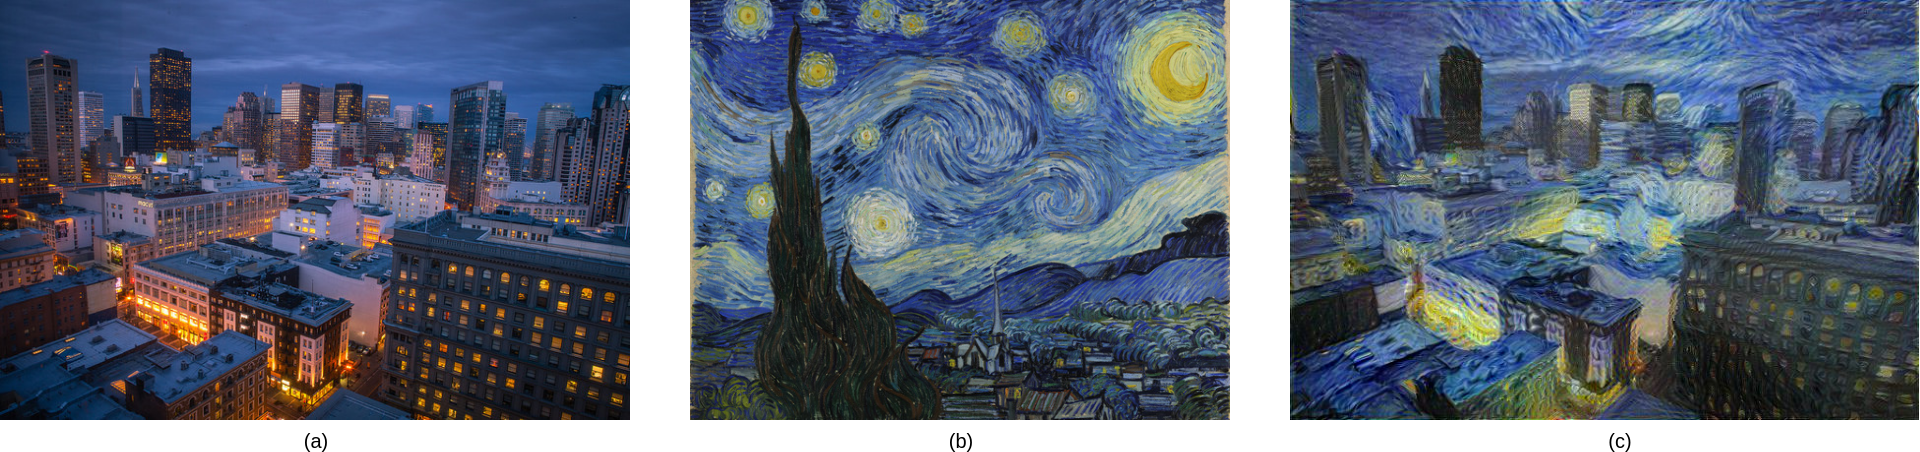
\includegraphics[width=.8\textwidth]{images/style-transfer-vision.png}
	\caption{\label{fig:style-transfer-vision}Sample of vision style transfer. Image (a) provides the content, image (b) provides the style and image (c) is the final generated image}
\end{figure}

This problem in the context of text was first introduced in 2012 \citep{xu2012paraphrasing} as a statistical model that attempted to paraphrase bodies of text in a different style using a simple replacement strategy. An few examples from this paper are shown in Table \ref{table:paraphrasing-for-style-results}. Since the overwhelming adopting of neural network based models in the language community, there have been many more works which break new ground in this area.

\begin{table}[ht]
	\centering
	\begin{tabular}{ | p{.45\linewidth} | p{.45\linewidth} | }
		\hline
		\textbf{Input}                                              & \textbf{Output}                                      \\
		\hline \hline
		i will bite thee by the ear for that jest .                 & i ’ ll bite you by the ear for that joke .           \\
		\hline
		what further woe conspires against mine age ?               & what ’ s true despair conspires against my old age ? \\
		\hline
		how doth my lady ?                                          & how is my lady ?                                     \\
		\hline
		hast thou slain tybalt ?                                    & have you killed tybalt ?                             \\
		\hline
		an i might live to see thee married once , i have my wish . & if i could live to see you married, i ’ ve my wish . \\
		\hline
		benvolio , who began this bloody fray ?                     & benvolio , who started this bloody fight itself ?    \\
		\hline
		what is your will ?                                         & what do you want ?                                   \\
		\hline
		call her forth to me .                                      & bring her out to me .                                \\
		\hline
	\end{tabular}
	\label{table:paraphrasing-for-style-results}
	\caption{Results of transferring authorship style from Shakespearan plays to modern english}
\end{table}


\section{Problem Statement}

The problem this thesis tackles is to perform an exploratory analysis of previous methods and test novel hypotheses to obtain neural disentanglement of latent spaces and its applications to linguistic style transfer.

We operate under the following constraints and assumptions in our formulation of the problem:

\begin{itemize}
	\item The model is singular, with no conditional execution branch based on desired attribute. i.e. there is only one decoder and the number of decoders does not scale with the number of distinct transferrable attributes.
	\item The corpus of styles are non-parallel i.e. for instance, there are no pairs of \texttt{$(document_1, document_2)$} for $styles \in (1, 2)$, as would be commonly seen in neural machine translation corpora.
	\item The corpora is annotated with the current attribute each document possesses e.g. each document has a corresponding 'positive'/'negative' label if the task is to do sentiment transfer.
	\item Optionally, a lexicon of words that are statistically very likely to be associated with each distict class label would be useful, primarily to evaluate how well content has been preserved without penalizing change in vocabulary caused by the transferring of style.
\end{itemize}
